\section{条件概率}
\label{sec:cprob-conditional}

掷两枚骰子，第一枚是六点的概率是$1/6$。若有人看了一眼，告诉我们“点数和不小于$9$”，第一枚是六点的可能性还是$1/6$吗？直觉上应该更大，点数和大，说明骰子点数偏高。已知信息排除了一部分结果，剩余不确定性应当只在留下的结果中描述。

\paragraph{缩小范围，重新归一}
令$A$为“第一枚是六点”，$B$为“点数和不小于$9$”。$B$包含点数和为$9,10,11,12$的格子，个数分别是$4,3,2,1$，共$10$个；其中第一枚是六点的有$(6,3),(6,4),(6,5),(6,6)$这$4$个，如图~\ref{fig:cprob-conditioning-shrink}所示。

既然知道结果落在$B$中，$B$之外的$26$个格子就不必再考虑。原来$36$个结果等可能，留下的$10$个结果之间也没有理由偏向哪个，所以把它们看成新的等可能样本空间，每格的概率从$1/36$变为$1/10$。在这个缩小的范围里，$A$占$4$格，可能性是$4/10=2/5$。

\begin{BookInlineFigure}
  \centering
  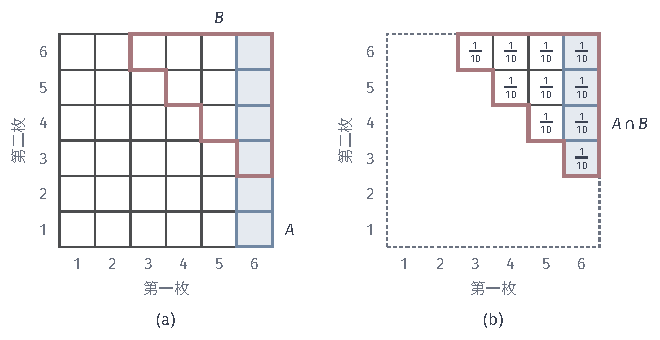
\includegraphics[width=112mm]{figures/07-probability/01-elementary-probability/tikz/cprob-conditioning-shrink/figure.pdf}
  \caption{以“点数和不小于$9$”为条件。(a)红线围出条件事件$B$的$10$个格子，浅蓝一列是$A$（第一枚六点），每格概率$1/36$。(b)只保留$B$中的格子，每格重新分得$1/10$；浅蓝格子是$A\cap B$，共$4$格，条件概率为$4/10$。}
  \label{fig:cprob-conditioning-shrink}
\end{BookInlineFigure}

把这个计算写成概率的形式。在古典模型中，
\[
 \frac{\lvert A\cap B\rvert}{\lvert B\rvert}
 =\frac{\lvert A\cap B\rvert/\lvert\Omega\rvert}{\lvert B\rvert/\lvert\Omega\rvert}
 =\frac{\mathbb{P}(A\cap B)}{\mathbb{P}(B)}.
\]
右端不再提到计数，只用到事件的概率，因此可以作为一般的定义。

\begin{definition}[条件概率]
\label{def:cprob-conditional}
设事件$B$满足$\mathbb{P}(B)>0$。事件$A$在$B$发生条件下的\term{条件概率}（conditional probability）定义为
\begin{equation}
 \mathbb{P}(A\mid B)=\frac{\mathbb{P}(A\cap B)}{\mathbb{P}(B)}.
 \label{eq:cprob-conditional}
\end{equation}
\end{definition}

分子只保留$A$中同时落在$B$内的部分，分母把$B$的概率重新标定为$1$。用质量的图景说：把$B$之外的质量全部清除，再把$B$内的质量按原有比例放大，使总量回到$1$。$B$内各点之间的相对大小不变，这正是“已知$B$发生”所允许的全部修改。

条件$\mathbb{P}(B)>0$不能去掉。在有限的古典模型中，$\mathbb{P}(B)=0$意味着$B=\varnothing$，以一个不可能发生的事件为条件没有意义，式~\eqref{eq:cprob-conditional}的分母也为零。

\paragraph{条件概率仍是概率}
固定$B$以后，$A\mapsto\mathbb{P}(A\mid B)$给每个事件分配了一个数。它满足前面的三条基本性质，因而第~\ref{sec:cprob-computing}节的补事件公式、加法公式在条件之下都可以照用。

\begin{theorem}[条件概率的基本性质]
\label{thm:cprob-conditional-axioms}
设$\mathbb{P}(B)>0$，则对任意事件$A,A'$，
\begin{equation}
 \mathbb{P}(A\mid B)\geq0,\qquad \mathbb{P}(\Omega\mid B)=1,
 \label{eq:cprob-conditional-normalized}
\end{equation}
并且当$A\cap A'=\varnothing$时，
\begin{equation}
 \mathbb{P}(A\cup A'\mid B)=\mathbb{P}(A\mid B)+\mathbb{P}(A'\mid B).
 \label{eq:cprob-conditional-additive}
\end{equation}
\end{theorem}

\begin{proof}
非负性来自分子非负、分母为正。由$\Omega\cap B=B$，分子分母相同，所以$\mathbb{P}(\Omega\mid B)=1$。若$A\cap A'=\varnothing$，则$A\cap B$与$A'\cap B$也互斥，且它们的并是$(A\cup A')\cap B$。由式~\eqref{eq:cprob-additive}，
\[
 \mathbb{P}\bigl((A\cup A')\cap B\bigr)=\mathbb{P}(A\cap B)+\mathbb{P}(A'\cap B).
\]
两边同除以$\mathbb{P}(B)$，就得到式~\eqref{eq:cprob-conditional-additive}。
\end{proof}

例如在上面的骰子例子中，$\mathbb{P}(A^{\mathrm{c}}\mid B)=1-2/5=3/5$，即已知点数和不小于$9$时，第一枚不是六点的概率是$3/5$。

\paragraph{两个方向的条件概率}
$\mathbb{P}(A\mid B)$与$\mathbb{P}(B\mid A)$的分子相同，都是$\mathbb{P}(A\cap B)$，分母不同。在骰子例子中，
\[
 \mathbb{P}(A\mid B)=\frac{4/36}{10/36}=\frac25,\qquad
 \mathbb{P}(B\mid A)=\frac{4/36}{6/36}=\frac23.
\]
前者是“点数和大时，第一枚是六点的概率”，后者是“第一枚是六点时，点数和大的概率”。它们回答不同的问题，一般不相等。把两者混为一谈是条件概率中最常见的错误，后面的检测例子会显示它可以造成多大的偏差。

已知$B$让$A$的概率从$1/6$升到$2/5$，这是信息的作用。条件概率也可能比原概率小，例如已知“点数和不大于$4$”时，第一枚是六点的概率降为$0$。若条件概率与原概率相等，条件就没有改变$A$的可能性，这种情形在第~\ref{sec:cprob-independence}节研究。

\subsection{乘法规则}
\label{sec:cprob-multiplication-rule}

很多试验是分步进行的：先摸第一个球，再摸第二个；先选产线，再看产品是否合格。每一步的条件概率往往可以直接从当时的物理状态读出，而整个样本空间却不必列出。把定义~\eqref{eq:cprob-conditional}反过来用，就能把这些逐步的概率乘起来。

\paragraph{两步乘法}
式~\eqref{eq:cprob-conditional}两边乘以$\mathbb{P}(B)$，得到
\begin{equation}
 \mathbb{P}(A\cap B)=\mathbb{P}(B)\,\mathbb{P}(A\mid B),\qquad \mathbb{P}(B)>0.
 \label{eq:cprob-multiplication}
\end{equation}
这称为概率的\term{乘法规则}（multiplication rule）。它的含义是比例的比例：$B$占全体的比例，乘以$A$在$B$内部所占的比例，等于$A\cap B$占全体的比例。

回到摸球问题，令$H_i$为“第$i$个球是黑球”。第一个球是黑球的概率是$3/5$。第一个黑球摸走以后，盒中剩下$2$黑$2$白，所以$\mathbb{P}(H_2\mid H_1)=2/4$。由式~\eqref{eq:cprob-multiplication}，
\[
 \mathbb{P}(H_1\cap H_2)=\mathbb{P}(H_1)\,\mathbb{P}(H_2\mid H_1)=\frac35\cdot\frac24=\frac{3}{10}.
\]
这与第~\ref{sec:cprob-computing}节在有序记录中数出的$6/20$一致。

这里的$\mathbb{P}(H_2\mid H_1)=2/4$是从“已知第一个是黑球”这个条件下盒中的实际构成读出来的。若忽略条件的变化，把第二步也写成$3/5$，就会得到$9/25$，那是放回摸球的答案。不放回抽样中，每一步的条件概率都必须对应前面已经发生的结果。

\paragraph{树形图}
把所有分步的情形画出来，就得到图~\ref{fig:cprob-urn-tree}的树形图。从根出发，每一层是一步，分支上写的是在到达该分支之前的结果已知时的条件概率；从根到叶的一条路径是一个完整的结果，它的概率是路径上各分支概率的乘积。

\begin{BookInlineFigure}
  \centering
  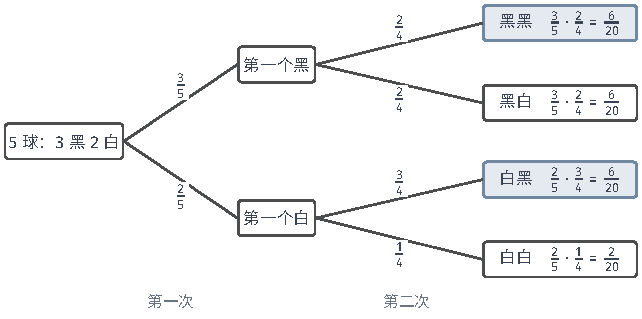
\includegraphics[width=109mm]{figures/07-probability/01-elementary-probability/tikz/cprob-urn-tree/figure.pdf}
  \caption{不放回摸两个球的树形图（盒中$3$黑$2$白）。分支上的数是条件概率，叶上是路径概率的乘积；四个叶的概率之和为$1$。浅蓝的两个叶组成事件$H_2$“第二个是黑球”。}
  \label{fig:cprob-urn-tree}
\end{BookInlineFigure}

同一个节点引出的分支，条件概率之和为$1$，这是式~\eqref{eq:cprob-conditional-normalized}的体现；因此全部叶的概率之和也是$1$。树形图上的叶就是颜色记录的四个结果，叶上的数与图~\ref{fig:cprob-urn-records}(c)一致。

\paragraph{多步乘法}
步骤更多时，反复使用式~\eqref{eq:cprob-multiplication}即可。

\begin{theorem}[多步乘法规则]
\label{thm:cprob-chain-rule}
设事件$A_1,\ldots,A_n$满足$\mathbb{P}(A_1\cap\cdots\cap A_{n-1})>0$，则
\begin{equation}
 \mathbb{P}(A_1\cap\cdots\cap A_n)
 =\mathbb{P}(A_1)\prod_{k=2}^{n}\mathbb{P}(A_k\mid A_1\cap\cdots\cap A_{k-1}).
 \label{eq:cprob-chain-rule}
\end{equation}
\end{theorem}

\begin{proof}
记$C_k=A_1\cap\cdots\cap A_k$。由包含关系$C_{n-1}\subseteq C_{n-2}\subseteq\cdots\subseteq C_1$与式~\eqref{eq:cprob-monotone}，各$\mathbb{P}(C_k)\geq\mathbb{P}(C_{n-1})>0$，右端每个条件概率都有定义。由定义~\eqref{eq:cprob-conditional}与$C_{k-1}\cap A_k=C_k$，
\[
 \mathbb{P}(A_k\mid C_{k-1})=\frac{\mathbb{P}(C_k)}{\mathbb{P}(C_{k-1})},\qquad k=2,\ldots,n,
\]
所以右端是
\[
 \mathbb{P}(C_1)\cdot\frac{\mathbb{P}(C_2)}{\mathbb{P}(C_1)}\cdot\frac{\mathbb{P}(C_3)}{\mathbb{P}(C_2)}\cdots\frac{\mathbb{P}(C_n)}{\mathbb{P}(C_{n-1})}.
\]
相邻的分子分母逐个相消，只剩$\mathbb{P}(C_n)$，即左端。
\end{proof}

用它重新计算第~\ref{sec:cprob-computing}节的扑克牌问题。令$R_k$为“第$k$张是红桃”。第一张是红桃的概率是$13/52$；已知第一张是红桃，剩下$51$张中有$12$张红桃；已知前两张都是红桃，剩下$50$张中有$11$张。由式~\eqref{eq:cprob-chain-rule}，
\[
 \mathbb{P}(R_1\cap R_2\cap R_3)=\frac{13}{52}\cdot\frac{12}{51}\cdot\frac{11}{50}=\frac{1716}{132600}=\frac{11}{850}.
\]
这与组合计数$\binom{13}{3}/\binom{52}{3}$的结果相同。组合计数一次数完整个样本空间，乘法规则则沿抽取过程逐步计算，每一步只需看当时剩下什么。

\subsection{全概率与Bayes公式}
\label{sec:cprob-total-bayes}

一家工厂有甲、乙、丙三条产线，某天生产的$1000$件产品中，甲线$500$件、乙线$300$件、丙线$200$件，次品分别有$10$件、$12$件、$20$件。从这$1000$件中随机抽一件，它是次品的概率是多少？如果它是次品，它最可能来自哪条产线？前一个问题按来源分组再合计，后一个问题从结果反推来源。

\paragraph{按情形分组}
令$L_1,L_2,L_3$分别为“抽到的产品来自甲、乙、丙线”，$D$为“抽到的是次品”。每件产品恰好来自一条产线，所以$L_1,L_2,L_3$两两互斥，并且它们的并是$\Omega$。这样一组事件称为样本空间的一个\term{划分}（partition）：每次试验中恰有一个$L_i$发生。

每条产线的比例和次品率可以直接读出：
\[
 \mathbb{P}(L_1)=0.5,\quad \mathbb{P}(L_2)=0.3,\quad \mathbb{P}(L_3)=0.2,
\]
\[
 \mathbb{P}(D\mid L_1)=\frac{10}{500}=0.02,\qquad
 \mathbb{P}(D\mid L_2)=\frac{12}{300}=0.04,
\]
\[
 \mathbb{P}(D\mid L_3)=\frac{20}{200}=0.10.
\]
要得到$\mathbb{P}(D)$，把$D$按来源切成三块，分别用乘法规则计算，再相加。

\begin{theorem}[全概率公式]
\label{thm:cprob-total-probability}
设$L_1,\ldots,L_m$是样本空间的一个划分，且每个$\mathbb{P}(L_i)>0$。则对任意事件$D$，
\begin{equation}
 \mathbb{P}(D)=\sum_{i=1}^{m}\mathbb{P}(L_i)\,\mathbb{P}(D\mid L_i).
 \label{eq:cprob-total-probability}
\end{equation}
\end{theorem}

\begin{proof}
由$L_1\cup\cdots\cup L_m=\Omega$，得$D=(D\cap L_1)\cup\cdots\cup(D\cap L_m)$；由$L_i$两两互斥，各块$D\cap L_i$也两两互斥。由有限个事件的互斥可加性，
\[
 \mathbb{P}(D)=\sum_{i=1}^{m}\mathbb{P}(D\cap L_i).
\]
对每一项用乘法规则~\eqref{eq:cprob-multiplication}，把$\mathbb{P}(D\cap L_i)$写成$\mathbb{P}(L_i)\mathbb{P}(D\mid L_i)$，代入即得。
\end{proof}

式~\eqref{eq:cprob-total-probability}称为\term{全概率公式}（law of total probability）。它是一个加权平均：各组的次品率$\mathbb{P}(D\mid L_i)$按各组所占的比例$\mathbb{P}(L_i)$加权。代入产线的数据，
\[
 \mathbb{P}(D)=0.5\times0.02+0.3\times0.04+0.2\times0.10=0.010+0.012+0.020=0.042.
\]
这正是$1000$件中次品所占的比例$42/1000$。

图~\ref{fig:cprob-line-mosaic}(a)把这个加权平均画成面积。单位正方形按产线比例分成三列，每列底部深色条的高度是该线的次品率，深色条的面积就是$\mathbb{P}(D\cap L_i)$，三块面积之和是$\mathbb{P}(D)$。

\begin{BookInlineFigure}
  \centering
  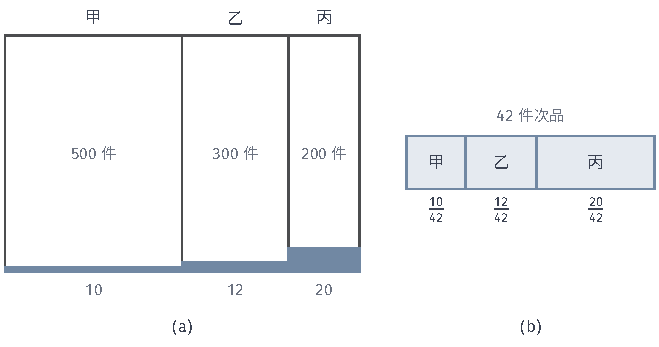
\includegraphics[width=112mm]{figures/07-probability/01-elementary-probability/tikz/cprob-line-mosaic/figure.pdf}
  \caption{三条产线的面积图，按真实比例绘制。(a)列宽是产线所占比例$0.5,0.3,0.2$，底部深蓝条的高度是次品率$0.02,0.04,0.10$，下方数字是各线次品件数；深蓝条的总面积是$\mathbb{P}(D)=0.042$。(b)只看$42$件次品，每件占同样长度，三段的比例就是$\mathbb{P}(L_i\mid D)$。}
  \label{fig:cprob-line-mosaic}
\end{BookInlineFigure}

\paragraph{从结果反推来源}
现在已知抽到的是次品，问它来自各条产线的概率。按定义，这是把范围缩小到$D$，在其中计算$L_i\cap D$所占的比例。分子用乘法规则写开，分母用全概率公式写开，就得到下面的公式。

\begin{theorem}[Bayes公式]
\label{thm:cprob-bayes}
在定理~\ref{thm:cprob-total-probability}的条件下，若$\mathbb{P}(D)>0$，则对每个$i$，
\begin{equation}
 \mathbb{P}(L_i\mid D)=\frac{\mathbb{P}(L_i)\,\mathbb{P}(D\mid L_i)}{\sum_{j=1}^{m}\mathbb{P}(L_j)\,\mathbb{P}(D\mid L_j)}.
 \label{eq:cprob-bayes}
\end{equation}
\end{theorem}

\begin{proof}
由定义~\eqref{eq:cprob-conditional}与乘法规则~\eqref{eq:cprob-multiplication}，
\[
 \mathbb{P}(L_i\mid D)=\frac{\mathbb{P}(L_i\cap D)}{\mathbb{P}(D)}=\frac{\mathbb{P}(L_i)\,\mathbb{P}(D\mid L_i)}{\mathbb{P}(D)}.
\]
再用全概率公式~\eqref{eq:cprob-total-probability}代入分母即得。
\end{proof}

式~\eqref{eq:cprob-bayes}称为\term{Bayes公式}（Bayes' formula）。分子就是图~\ref{fig:cprob-line-mosaic}(a)中第$i$块深色条的面积，分母是三块面积之和。代入数据，
\[
 \mathbb{P}(L_1\mid D)=\frac{0.010}{0.042}=\frac{10}{42},\quad
 \mathbb{P}(L_2\mid D)=\frac{12}{42},\quad
 \mathbb{P}(L_3\mid D)=\frac{20}{42}\approx0.476.
\]
在古典模型中这就是在$42$件次品里数各产线的件数，图~\ref{fig:cprob-line-mosaic}(b)把这$42$件单独排开。

\paragraph{先验与后验}
Bayes公式中的两组比例含义不同。$\mathbb{P}(L_i)$是抽到产品之前、不知道它是否为次品时对来源的估计，称为\term{先验}（prior）概率；$\mathbb{P}(L_i\mid D)$是观察到“次品”之后的来源概率，称为\term{后验}（posterior）概率。$\mathbb{P}(D\mid L_i)$是各来源产生这一观察的可能性。

丙线只生产了$20\%$的产品，却占了次品的约$47.6\%$；甲线生产了一半，在次品中只占约$23.8\%$。后验把先验按“各来源产生观察的可能性”重新加权：次品率高的产线，在次品中的份额被放大。

若要把这件次品归到一条产线去追查，按后验概率最大的原则应归到丙线。这是用条件概率作分类：比较的是$\mathbb{P}(L_i\mid D)$，而不是$\mathbb{P}(L_i)$或$\mathbb{P}(D\mid L_i)$单独一项。若抽到的是合格品，同样的计算给出后验约为$0.512,0.301,0.188$，与先验相差不大，合格品几乎不提供来源的信息。

条件也可以反推时间上更早的结果。在摸球问题中，已知第二个球是黑球，第一个球是黑球的概率是多少？由图~\ref{fig:cprob-urn-tree}，$\mathbb{P}(H_2)=6/20+6/20=3/5$，于是
\[
 \mathbb{P}(H_1\mid H_2)=\frac{\mathbb{P}(H_1\cap H_2)}{\mathbb{P}(H_2)}=\frac{6/20}{12/20}=\frac12.
\]
第二个球不能影响第一个球是什么，但知道第二个球的颜色，会改变我们对第一个球的判断。条件概率描述的是信息，而不是因果。

\paragraph{条件要对应实际得到的信息}
用条件概率时，条件必须是实际知道的那个事件，而不是与它意思相近的另一个事件。下面的三扇门问题说明两者的差别。三扇门中的一扇后面有奖品，奖品在各扇门后的可能性相同。参赛者选了1号门；主持人知道奖品的位置，他从另外两扇门中打开一扇没有奖品的门，若两扇都没有奖品，就各以$1/2$的概率任选一扇。现在主持人打开了3号门，奖品在2号门后的概率是多少？

一种常见的回答是：3号门后没有奖品，剩下1号和2号两扇门，各占$1/2$。这个回答所用的条件是“奖品不在3号门后”，可我们实际看到的是“主持人打开了3号门”。后者比前者包含更多信息：奖品若在1号门后，主持人有两扇门可选；奖品若在2号门后，他只能打开3号门。

令$C_i$为“奖品在$i$号门后”，$O_3$为“主持人打开3号门”。$C_1,C_2,C_3$构成划分，各自的先验概率是$1/3$。由主持人的规则，
\[
 \mathbb{P}(O_3\mid C_1)=\frac12,\qquad \mathbb{P}(O_3\mid C_2)=1,\qquad \mathbb{P}(O_3\mid C_3)=0.
\]
由全概率公式与Bayes公式，
\[
 \mathbb{P}(O_3)=\frac13\Bigl(\frac12+1+0\Bigr)=\frac12,
\]
\[
 \mathbb{P}(C_2\mid O_3)=\frac{\frac13\cdot1}{\frac12}=\frac23,\qquad
 \mathbb{P}(C_1\mid O_3)=\frac{\frac13\cdot\frac12}{\frac12}=\frac13.
\]

图~\ref{fig:cprob-three-doors-tree}把四种情形画成树形图。红框的两片叶是“打开3号门”，它们的概率分别是$1/6$和$1/3$，后者是前者的两倍。所以换到2号门，得到奖品的概率是$2/3$。若主持人并不知道奖品位置、只是碰巧打开了一扇空门，$\mathbb{P}(O_3\mid C_2)$就变成$1/2$，答案也随之变成$1/2$。同样是“3号门后没有奖品”，信息产生的方式不同，条件事件就不同。

\begin{BookInlineFigure}
  \centering
  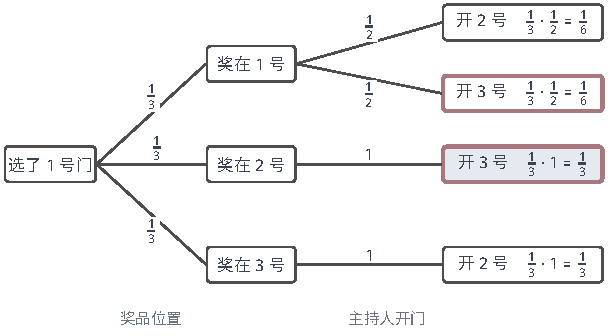
\includegraphics[width=103mm]{figures/07-probability/01-elementary-probability/tikz/cprob-three-doors-tree/figure.pdf}
  \caption{三扇门问题的树形图。第一层是奖品位置，第二层是主持人按规则开的门，分支上是条件概率，叶上是路径概率。红框的两片叶组成观察到的事件“打开3号门”，其中浅蓝的一片（奖在2号门后）占$\frac{1/3}{1/2}=\frac23$。}
  \label{fig:cprob-three-doors-tree}
\end{BookInlineFigure}

\paragraph{检测中的三个比例}
产品出厂前要经过一道自动检测。设某批产品中次品率为$2\%$；检测对次品报警的概率为$0.95$，对合格品误报的概率为$0.05$。一件产品报警了，它是次品的概率是多少？很多人会回答$0.95$，下面的计算说明这个答案错得很远。

令$D$为“次品”，$T$为“报警”。已知量是
\[
 \mathbb{P}(D)=0.02,\qquad \mathbb{P}(T\mid D)=0.95,\qquad \mathbb{P}(T\mid D^{\mathrm{c}})=0.05.
\]
$D$与$D^{\mathrm{c}}$构成划分。由全概率公式，报警的概率是
\[
 \mathbb{P}(T)=0.02\times0.95+0.98\times0.05=0.019+0.049=0.068.
\]
由Bayes公式，
\[
 \mathbb{P}(D\mid T)=\frac{0.019}{0.068}=\frac{19}{68}\approx0.279.
\]

图~\ref{fig:cprob-test-frequency-tree}用$10000$件产品把这些比例换成件数。$200$件次品中有$190$件报警，$9800$件合格品中有$490$件误报；报警的$680$件里只有$190$件是次品。误报率虽小，合格品的数量却大得多，误报的件数反而超过了真正的次品。

\begin{BookInlineFigure}
  \centering
  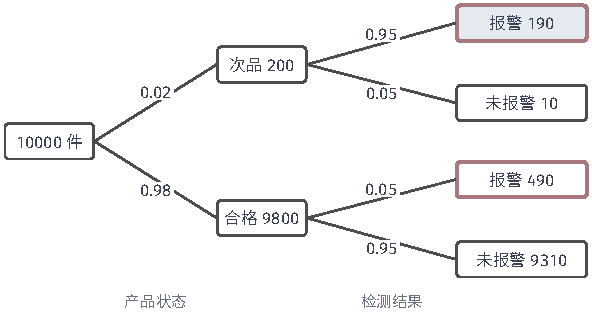
\includegraphics[width=100mm]{figures/07-probability/01-elementary-probability/tikz/cprob-test-frequency-tree/figure.pdf}
  \caption{用$10000$件产品表示检测的各个比例。分支上的数是条件概率，节点中是件数；红框是报警的两组，浅蓝的一组是报警且为次品，占报警件数的$190/680\approx0.279$。}
  \label{fig:cprob-test-frequency-tree}
\end{BookInlineFigure}

这个例子中三个数分别回答三个问题：先验比例$\mathbb{P}(D)=0.02$是检测前一件产品为次品的概率；条件检出概率$\mathbb{P}(T\mid D)=0.95$描述检测的性能，即在次品中报警的比例；后验比例$\mathbb{P}(D\mid T)\approx0.279$是在报警的产品中次品的比例。第二个与第三个的分子相同、分母不同，正是前面说的两个方向的条件概率。

\paragraph{信息的逐次更新}
报警的产品再送去复检一次。设复检用同样性能的设备，并假设：对给定状态的产品，复检是否报警不受第一次结果的影响，即
\[
 \mathbb{P}(T_2\mid D\cap T_1)=\mathbb{P}(T_2\mid D)=0.95,\qquad
 \mathbb{P}(T_2\mid D^{\mathrm{c}}\cap T_1)=\mathbb{P}(T_2\mid D^{\mathrm{c}})=0.05,
\]
其中$T_1,T_2$分别是两次报警。若两次报警之后才判定，次品的概率是多少？

已知$T_1$发生，就在$\mathbb{P}(\cdot\mid T_1)$下计算。由定理~\ref{thm:cprob-conditional-axioms}，它满足三条基本性质，所以全概率公式与Bayes公式对它同样成立。在它之下再以$D$为条件，得到的正是以$D\cap T_1$为条件：
\[
 \frac{\mathbb{P}(T_2\cap D\mid T_1)}{\mathbb{P}(D\mid T_1)}
 =\frac{\mathbb{P}(T_2\cap D\cap T_1)/\mathbb{P}(T_1)}{\mathbb{P}(D\cap T_1)/\mathbb{P}(T_1)}
 =\mathbb{P}(T_2\mid D\cap T_1).
\]
因此公式中的先验换成第一次报警后的后验$19/68$，条件检出概率换成上面假设的$\mathbb{P}(T_2\mid D\cap T_1)$与$\mathbb{P}(T_2\mid D^{\mathrm{c}}\cap T_1)$：
\[
 \mathbb{P}(D\mid T_1\cap T_2)
 =\frac{\frac{19}{68}\times0.95}{\frac{19}{68}\times0.95+\frac{49}{68}\times0.05}
 =\frac{18.05}{18.05+2.45}=\frac{361}{410}\approx0.880.
\]
一次观察后的后验成为下一次观察的先验，信息就这样逐次累积。

比值的写法更能看出每次更新做了什么。次品与合格品的概率之比，先验是$0.02:0.98=1:49$。由式~\eqref{eq:cprob-bayes}，两个后验的分母相同，比值只由分子决定：
\begin{equation}
 \frac{\mathbb{P}(D\mid T)}{\mathbb{P}(D^{\mathrm{c}}\mid T)}
 =\frac{\mathbb{P}(D)}{\mathbb{P}(D^{\mathrm{c}})}\cdot\frac{\mathbb{P}(T\mid D)}{\mathbb{P}(T\mid D^{\mathrm{c}})}.
 \label{eq:cprob-odds}
\end{equation}
右端第二个因子称为观察$T$的\term{似然比}（likelihood ratio），这里是$0.95/0.05=19$。每次报警把比值乘以$19$：一次后为$19:49$，即概率$19/68$；两次后为$361:49$，即概率$361/410$。

图~\ref{fig:cprob-posterior-prior}把后验画成先验次品率的函数。先验很小时，一次报警之后的后验仍然不大；同一个似然比作用在不同的先验上，结果可以相差很多。这再次说明，只知道检测的性能，不知道先验比例，无法回答“报警的产品有多大可能是次品”。

\begin{BookInlineFigure}
  \centering
  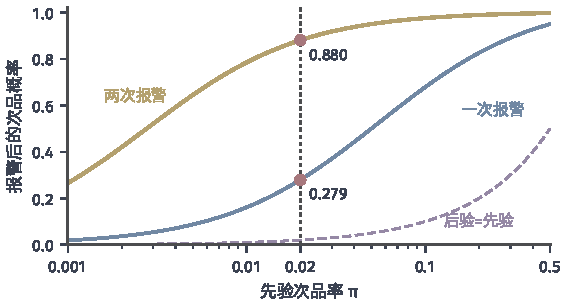
\includegraphics[width=96mm]{figures/07-probability/01-elementary-probability/matplotlib/cprob-posterior-prior/figure.pdf}
  \caption{报警后为次品的概率随先验次品率$\pi$的变化，横轴为对数坐标。检出概率$0.95$，误报概率$0.05$。蓝线是一次报警后的后验，黄线是两次报警后的后验（假设给定状态时两次检测互不影响），紫色虚线是后验等于先验的参考线；红点标出正文中$\pi=0.02$的两个值。}
  \label{fig:cprob-posterior-prior}
\end{BookInlineFigure}

两次更新所用的假设必须核对。如果某类次品的缺陷检测设备根本看不出来，第一次漏报的产品第二次也会漏报，两次结果就不再互不影响，乘以两次似然比会高估证据的强度。这个假设是对条件概率$\mathbb{P}(\cdot\mid D)$与$\mathbb{P}(\cdot\mid D^{\mathrm{c}})$的要求，下一节会看到它与“两次报警互不影响”并不是一回事。
